The prototype application developed for this FYP was created for use on an Android device.

\subsection*{Activity Lifecycle}
An activity in an Android application represents a single UI screen.
As a user navigates an application, the activities within the application go through different stages of their lifecycle \parencite{android}.
The stages in an activities lifecycle can be seen in Figure \ref{fig:android}.

\begin{figure}[h]
    \centering
    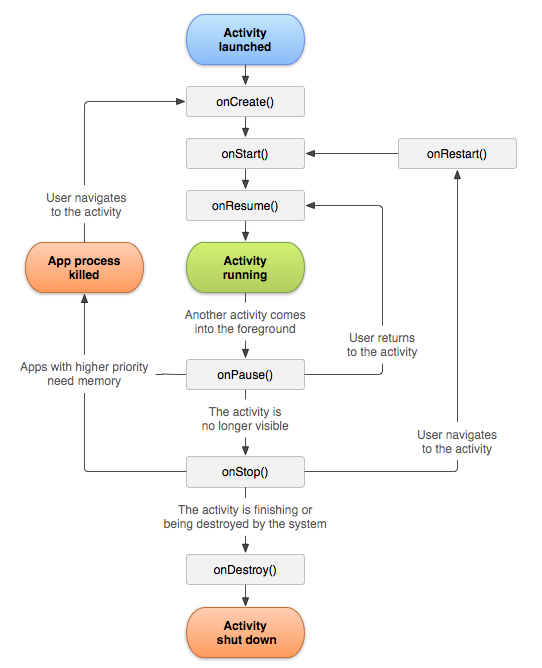
\includegraphics[scale=0.5]{android}
    \caption{Android Activity Lifecycle \parencite{android}}
    \label{fig:android}
\end{figure}

Android provides call back mechanisms for each stage of the lifecycle.
These call backs are:
\begin{itemize}
	\item{onCreate(): This callback is executed when the activity is first created and must be implemented.}
	\item{onStart(): This callback is triggered when the activity is in the Started state. This callback executes the code that prepares the UI for use.}
	\item{onResume(): This callback is triggered when the activity is resumed. This could occur if the user temporarily leaves the activity and returns.}
	\item{onPause(): This callback is invoked when a user is leaving an activity to be returned to later.}
	\item{onStop(): This callback is executed when the activity is finished running or is no longer accessible by the user.}
	\item{onDestroy(): The onDestroy() callback is invoked before the activity is destroyed and it is the final callback executed.}
\end{itemize}

\subsection*{Android Studio}
Android Studio is an IDE that is very common for the development of Android applications.
It is developed by JetBrains who also created the InteliJ IDE and there are many similarities between the two.
Android Studio provides a nice interface for the creation of the user interface of applications with a drag and drop mechanism.

\subsection*{Languages}
There are two main languages used for Android development in the Android Studio IDE are Java and Kotlin.
Kotlin is a language developed by JetBrains with the tag line of "Statically typed programming language for modern multiplatform applications" \parencite{kotlin}.
It is defined as being safe, tool-friendly, inter-operable and concise by the reduction of boilerplate (repetitive) code.

\subsection*{Key Concepts}
In the development of Android applications an intent can be used as an abstraction to execute operations.
Intents can launch activities, communicate with services running in the background and can also initiate broadcast receivers (allows use of system resources).

An AsyncTask in an abstract class in Android development.
Its enables the performance of background operations and to call the UI thread with ease.
They are aimed towards short operations which take a few seconds at most.

In Android development, an onClickListener is used to define actions for when a view is clicked.
It is an interface that is implemented as a callback for when views are clicked.